\documentclass[a4paper]{ctexart}
\usepackage{amsmath}
\usepackage{amsthm}
\usepackage{enumerate}
\usepackage{graphicx}
\usepackage{lmodern}
\usepackage[textwidth=14.5cm]{geometry}
\usepackage{blindtext}
\parindent=0pt

\title{算法分析与设计 - HW3}
\author{}
\date{2022/10/06}

\begin{document}
\begin{sloppypar}

    \maketitle

    n个铁管具有重量, 被按序存放在$w[i] (1 \leq i \leq n)$.
    这些铁管将根据它们的顺序, 被焊接成一个大的铁管,
    每个时间任意两个相邻的铁管可以被选中来进行焊接.
    焊接的代价是焊接的铁管中的重量较大的铁管的重量. \\
    例如: $w[1]=5, w[2]=1, w[3]=2$, 如果1和2先进行焊接,
    则焊接的代价为5, 然后3被焊接代价为6, 那么总的焊接代价为$5 + 5=10$.
    但是如果先焊接2和3,再焊1, 那么总的代价为$2 + 5=7$.
    \begin{enumerate}[(1)]
        \item 设计一个动态规划算法去发现最优的焊接顺序,
              使得整个代价最小和确立迭代关系. \\
              \textbf{解:} \\
              伪代码如下:
              \begin{figure}[h]
                  \centering
                  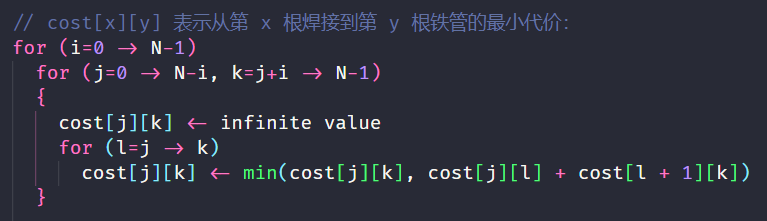
\includegraphics[scale=0.8]{pseudo_code.png}
              \end{figure}

        \item 将设计的算法应用到一个具体的实例中,
              去发现最优焊接顺序和其相应的焊接总代价, 该实例具有5个钢管:
              $w[1]=6, w[2]=2, w[3]=7, w[4]=5, w[5]=8$.
              请给出详细的解决过程. \\
              \textbf{解:} \\
              第一轮计算代价: \\
              $cost[1][2]=6, cost[2][3]=7, cost[3][4]=7, cost[4][5]=8$ \\
              第二轮计算代价: \\
              $cost[1][3]=min(6+7, 6+7)=13, cost[2][4]=min(7+5, 2+7)=9, cost[3][5]=min(7+8, 7+8)=15$ \\
              第三轮计算代价: \\
              $cost[1][4]=min(6+9, 6+7, 13+5)=13, cost[2][5]=min(2+15, 7+8, 9+8)=15$
              第四轮计算代价: \\
              $cost[1][5]=min(6+15, 6+15, 13+8, 13+8)=21$
    \end{enumerate}

\end{sloppypar}
\end{document}
